% ============================================================
%  DjerbaStay — Cahier des Charges (PFA 2025-2026)
%  Compile with : pdflatex  (×2 for TOC)
% ============================================================
\documentclass[12pt,a4paper]{report}

% ---------- packages ----------
\usepackage[utf8]{inputenc}
\usepackage[T1]{fontenc}
\usepackage[french]{babel}
\usepackage{geometry}
\geometry{margin=2.5cm}
\usepackage{graphicx}
\usepackage{array}
\usepackage{booktabs}
\usepackage{longtable}
\usepackage{enumitem}
\usepackage{hyperref}
\usepackage{xcolor}
\usepackage{titlesec}
\usepackage{fancyhdr}
\usepackage{tabularx}
\usepackage{float}

% ---------- style ----------
\hypersetup{
  colorlinks  = true,
  linkcolor   = blue!60!black,
  urlcolor    = blue!60!black,
  citecolor   = blue!60!black
}

\pagestyle{fancy}
\fancyhf{}
\fancyhead[L]{\small DjerbaStay --- Cahier des Charges}
\fancyhead[R]{\small PFA 2025--2026}
\fancyfoot[C]{\thepage}
\renewcommand{\headrulewidth}{0.4pt}

\titleformat{\chapter}[display]
  {\normalfont\Large\bfseries}{}{0pt}{\Large}
\titlespacing*{\chapter}{0pt}{-20pt}{20pt}

% ============================================================
\begin{document}

% ==================== PAGE DE GARDE ==========================
\begin{titlepage}
  \centering
  \vspace*{1cm}

  {\large République Tunisienne}\\[4pt]
  {\large Ministère de l'Enseignement Supérieur et de la Recherche Scientifique}\\[4pt]
  {\large Institut Supérieur d'Informatique et de Mathématiques}\\[2cm]

  \rule{\textwidth}{1pt}\\[0.6cm]
  {\Huge\bfseries CAHIER DES CHARGES}\\[0.3cm]
  {\Large Projet de Fin d'Année (PFA)}\\[0.6cm]
  \rule{\textwidth}{1pt}\\[1.5cm]

  {\LARGE\bfseries DjerbaStay}\\[0.5cm]
  {\large Planification intelligente d'activités touristiques à Djerba\\
  avec estimation de budget et suggestions personnalisées\\
  basées sur l'hébergement choisi}\\[2.5cm]

  \begin{tabular}{ll}
    \textbf{Réalisé par :} & Seif Balbali \\
                           & Mahdi Saadoui \\
                           & Majid Abdel Ali \\
                           & Mahmoud Balbali \\
                           & Sana Korbi \\[0.6cm]
    \textbf{Encadrant :}   & Nefaa Haffar \\[0.6cm]
    \textbf{Année universitaire :} & 2025 -- 2026 \\
    \textbf{Date :}        & 18 mars 2026 \\
  \end{tabular}

  \vfill
\end{titlepage}

% ==================== TABLE DES MATIERES =====================
\tableofcontents
\newpage

% ============================================================
%                    1.  PRESENTATION DU PROJET
% ============================================================
\chapter{Présentation du projet}

% ---- 1.1 Contexte général ---------------------------------
\section{Contexte général}

Djerba est une île touristique de premier plan en Tunisie. Chaque année, des
milliers de voyageurs --- étudiants, familles, touristes --- cherchent à
planifier un séjour sur l'île. Cependant, ils se heurtent à plusieurs
difficultés~:

\begin{itemize}
  \item Les voyageurs qui se rendent à Djerba ont du mal à planifier leurs
        activités quotidiennes en fonction de leur hébergement et de leur budget.
  \item Il est difficile de connaître à l'avance les distances entre les
        activités et l'hébergement choisi, ce qui complique l'organisation du
        séjour.
  \item La recherche manuelle d'activités sur plusieurs plateformes prend du
        temps et ne tient pas compte des préférences ni du profil du voyageur.
\end{itemize}

Le projet \textbf{DjerbaStay} s'inscrit dans ce contexte en proposant une
application web intelligente qui centralise ces informations et guide
l'utilisateur dans la planification de son séjour.

% ---- 1.2 Problématique ------------------------------------
\section{Problématique}

Les voyageurs qui se rendent à Djerba ont du mal à planifier leurs activités
quotidiennes en fonction de leur hébergement et de leur budget. Il est
difficile de connaître à l'avance les distances entre les activités et
l'hébergement choisi, ce qui complique l'organisation du séjour. La recherche
manuelle d'activités sur plusieurs plateformes prend du temps et ne tient pas
compte des préférences ni du profil du voyageur.

Une application intelligente peut automatiser cette planification en proposant
un programme journalier adapté, avec estimation de budget et informations de
proximité.

% ---- 1.3 Public cible -------------------------------------
\section{Public cible}

\begin{itemize}
  \item Étudiants en déplacement à Djerba.
  \item Touristes nationaux et internationaux souhaitant une planification
        simple, rapide et personnalisée de leur séjour.
  \item Voyageurs individuels souhaitant planifier un séjour à budget maîtrisé.
\end{itemize}

% ============================================================
%                    2.  OBJECTIFS DU PROJET
% ============================================================
\chapter{Objectifs du projet}

Le projet DjerbaStay vise à atteindre les objectifs suivants~:

\begin{enumerate}
  \item Permettre aux visiteurs de consulter les hébergements disponibles
        (hôtels et maisons d'hôtes) sans nécessiter de connexion.
  \item Proposer, après authentification, un modèle de recommandation
        d'activités journalières personnalisées selon le profil du voyageur.
  \item Calculer la distance entre chaque activité suggérée et l'hébergement
        sélectionné.
  \item Estimer le budget total du séjour et le budget par jour (hébergement +
        activités).
  \item Offrir aux administrateurs un tableau de bord pour gérer les
        hébergements et les utilisateurs.
  \item Fournir une interface web intuitive, simple et accessible depuis un
        navigateur web.
\end{enumerate}

% ============================================================
%                    3.  PERIMETRE DU PROJET
% ============================================================
\chapter{Périmètre du projet}

\section{Ce que le système inclut}

\begin{itemize}
  \item Inscription, connexion et gestion du profil utilisateur.
  \item Consultation et navigation sur le site (accès public).
  \item Visualisation de la liste des hébergements disponibles (hôtels et
        maisons d'hôtes).
  \item Module de recommandation d'activités journalières personnalisées (ML).
  \item Calcul des distances entre activités et hébergement.
  \item Module d'estimation du budget (total et par jour).
  \item Interface d'administration (gestion des utilisateurs et des données).
\end{itemize}

\section{Ce que le système n'inclut pas}

\begin{itemize}
  \item Le paiement en ligne ou la réservation directe.
  \item La couverture d'autres destinations en dehors de Djerba.
  \item Une application mobile native (iOS / Android).
\end{itemize}

% ============================================================
%            4.  DESCRIPTION DE LA SOLUTION
% ============================================================
\chapter{Description de la solution et valeur ajoutée}

\section{Accès public (sans connexion)}

\begin{itemize}
  \item Consultation et navigation sur le site.
  \item Visualisation de la liste des hébergements disponibles (hôtels et
        maisons d'hôtes).
\end{itemize}

\section{Authentification (inscription / connexion)}

\begin{itemize}
  \item Nécessaire pour accéder au modèle de recommandation.
  \item Inscription lors de la première visite, connexion pour les visites
        suivantes.
\end{itemize}

\section{Utilisation du modèle (utilisateur connecté)}

\begin{itemize}
  \item Sélection d'un hébergement depuis la liste disponible.
  \item Saisie du nombre de jours de séjour.
  \item Sélection du type de voyage (culturel, aventure, détente, famille, etc.).
  \item Indication des préférences personnelles supplémentaires.
\end{itemize}

\section{Résultats générés par le modèle}

\begin{itemize}
  \item Un programme d'activités suggérées pour chaque jour du séjour.
  \item La distance entre chaque activité et l'hébergement sélectionné.
  \item Une estimation du budget total et du budget par jour.
\end{itemize}

% ============================================================
%            5.  IDENTIFICATION DES ACTEURS
% ============================================================
\chapter{Identification des acteurs}

Le système fait intervenir deux acteurs principaux~:

\begin{table}[H]
\centering
\renewcommand{\arraystretch}{1.4}
\begin{tabularx}{\textwidth}{|l|l|X|}
\hline
\textbf{Acteur} & \textbf{Profil} & \textbf{Rôle dans le système} \\
\hline
Utilisateur (Visiteur / Touriste) & Non authentifié / Authentifié &
  Peut naviguer sur le site et consulter les hébergements sans connexion.
  Doit s'authentifier pour accéder au modèle de recommandation.
  Peut configurer son séjour et recevoir un programme personnalisé avec
  estimation de budget. \\
\hline
Administrateur & Gestionnaire de la plateforme &
  Accède à un tableau de bord dédié. Gère les hébergements (ajout,
  modification, suppression). Gère les comptes utilisateurs (consultation,
  activation, suppression). \\
\hline
\end{tabularx}
\caption{Identification des acteurs du système}
\end{table}

% ============================================================
%            6.  BESOINS FONCTIONNELS
% ============================================================
\chapter{Besoins fonctionnels}

Les besoins fonctionnels décrivent l'ensemble des fonctionnalités que le
système doit offrir.

\begin{longtable}{|c|p{8cm}|c|c|}
\hline
\textbf{ID} & \textbf{Description} & \textbf{Priorité} & \textbf{Acteur} \\
\hline
\endfirsthead
\hline
\textbf{ID} & \textbf{Description} & \textbf{Priorité} & \textbf{Acteur} \\
\hline
\endhead
BF-01 & L'utilisateur peut s'inscrire en fournissant ses informations
        personnelles (nom, email, mot de passe). & Haute & Visiteur \\
\hline
BF-02 & L'utilisateur peut se connecter et se déconnecter de son compte.
       & Haute & Visiteur / Utilisateur \\
\hline
BF-03 & L'utilisateur authentifié peut consulter et modifier son profil.
       & Moyenne & Utilisateur \\
\hline
BF-04 & Le visiteur peut parcourir le site et consulter la liste des
        hébergements disponibles. & Haute & Visiteur \\
\hline
BF-05 & L'utilisateur peut sélectionner un hébergement, saisir le nombre
        de jours, le type de voyage et ses préférences personnelles.
       & Haute & Utilisateur \\
\hline
BF-06 & Le système génère un programme d'activités journalières
        personnalisées grâce au module de Machine Learning.
       & Haute & Utilisateur \\
\hline
BF-07 & Le système calcule la distance entre chaque activité suggérée et
        l'hébergement sélectionné. & Haute & Utilisateur \\
\hline
BF-08 & Le système estime le budget total du séjour et le budget par jour
        (hébergement + activités). & Haute & Utilisateur \\
\hline
BF-09 & L'utilisateur peut consulter l'historique de ses recherches et
        résultats précédents. & Moyenne & Utilisateur \\
\hline
BF-10 & L'administrateur peut gérer les hébergements (ajout, modification,
        suppression). & Haute & Administrateur \\
\hline
BF-11 & L'administrateur peut gérer les comptes utilisateurs (consultation,
        activation, suppression). & Haute & Administrateur \\
\hline
BF-12 & L'administrateur peut surveiller les performances du module ML.
       & Moyenne & Administrateur \\
\hline
\end{longtable}

% ============================================================
%            7.  BESOINS NON FONCTIONNELS
% ============================================================
\chapter{Besoins non fonctionnels}

Les besoins non fonctionnels définissent les critères de qualité et les
contraintes techniques que le système doit respecter.

\begin{longtable}{|c|l|p{8cm}|}
\hline
\textbf{ID} & \textbf{Critère} & \textbf{Description} \\
\hline
\endfirsthead
\hline
\textbf{ID} & \textbf{Critère} & \textbf{Description} \\
\hline
\endhead
BNF-01 & Performance & Les résultats de recherche doivent s'afficher en moins
         de 3~secondes dans des conditions normales d'utilisation. \\
\hline
BNF-02 & Sécurité & Les mots de passe doivent être hachés (bcrypt). Les
         sessions doivent être gérées par des tokens sécurisés (JWT). Les
         données personnelles doivent être protégées. \\
\hline
BNF-03 & Disponibilité & Le système doit être disponible 24\,h/24 et 7\,j/7
         avec un taux de disponibilité minimal de 95\,\%. \\
\hline
BNF-04 & Compatibilité & L'interface doit être responsive et fonctionnelle sur
         les navigateurs modernes (Chrome, Firefox, Edge) ainsi que sur mobile
         et tablette. \\
\hline
BNF-05 & Maintenabilité & Le code source doit être modulaire, commenté et
         versionné (Git) afin de faciliter la maintenance et les évolutions
         futures. \\
\hline
BNF-06 & Scalabilité & Le système doit être conçu pour supporter une montée en
         charge progressive sans refonte majeure de l'architecture. \\
\hline
BNF-07 & Accessibilité & L'interface doit être en langue française, intuitive
         et utilisable sans formation préalable. \\
\hline
\end{longtable}

% ============================================================
%            8.  ARCHITECTURE TECHNIQUE
% ============================================================
\chapter{Architecture technique}

\section{Architecture générale}

Le projet s'appuie sur une architecture à quatre composants~:

\begin{enumerate}
  \item \textbf{Couche présentation (Frontend)}~: interface utilisateur
        accessible via un navigateur web.
  \item \textbf{Couche logique métier (Backend API)}~: traitement des requêtes,
        gestion des utilisateurs, des hébergements et de l'authentification.
  \item \textbf{Service ML séparé}~: recommandation d'activités journalières,
        calcul des distances entre activités et hébergement, estimation du
        budget total et par jour.
  \item \textbf{Couche données (Base de données)}~: stockage des informations
        relatives aux utilisateurs, hébergements et activités.
\end{enumerate}

\section{Technologies envisagées}

\begin{table}[H]
\centering
\renewcommand{\arraystretch}{1.4}
\begin{tabularx}{\textwidth}{|l|l|X|}
\hline
\textbf{Composant} & \textbf{Technologie} & \textbf{Rôle} \\
\hline
Frontend & Next.js + Tailwind CSS &
  Développement de l'interface utilisateur. \\
\hline
Backend principal & Node.js (Express.js) &
  API REST pour la gestion des utilisateurs, des hébergements et de
  l'authentification. \\
\hline
Service ML & Python + Flask &
  Recommandation d'activités, calcul des distances, estimation du budget. \\
\hline
Machine Learning & Scikit-learn, Pandas, NumPy &
  Entraînement et exécution du modèle de recommandation. \\
\hline
Base de données & PostgreSQL + Prisma (ORM) &
  Stockage et gestion des données (utilisateurs, hébergements, activités). \\
\hline
Données initiales & Fichier CSV &
  Importation initiale des hébergements et activités dans PostgreSQL. \\
\hline
Authentification & JSON Web Token (JWT) &
  Gestion sécurisée des sessions utilisateurs. \\
\hline
Versionnement & Git / GitHub &
  Suivi et collaboration sur le code source. \\
\hline
\end{tabularx}
\caption{Technologies envisagées}
\end{table}

% ============================================================
%  9.  DIAGRAMMES UML
% ============================================================
\chapter{Diagrammes UML}

% ---- 9.1 Diagramme de cas d'utilisation --------------------
\section{Diagramme de cas d'utilisation}

Le diagramme de cas d'utilisation ci-dessous illustre les interactions entre
les acteurs et le système.

\begin{figure}[H]
  \centering
  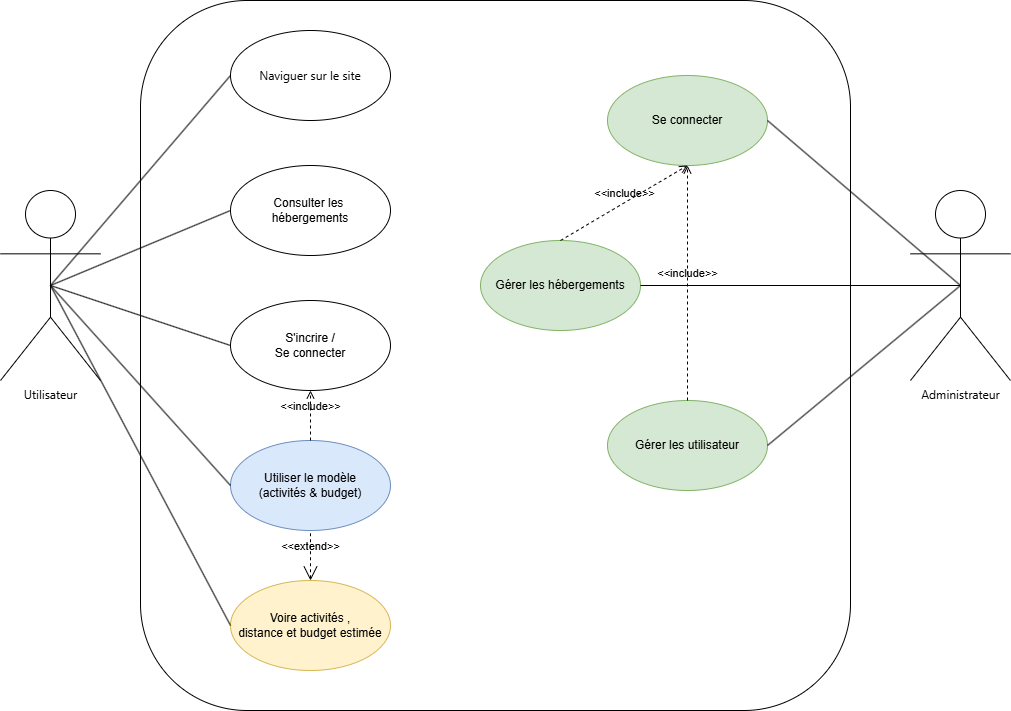
\includegraphics[width=0.85\textwidth]{use-case-pfa-without-bg.png}
  \caption{Diagramme de cas d'utilisation de DjerbaStay}
\end{figure}

\noindent
Le système identifie deux acteurs~:
\begin{itemize}
  \item \textbf{Utilisateur}~: peut naviguer sur le site, consulter les
        hébergements, s'inscrire / se connecter, utiliser le modèle
        (activités \& budget) et voir les activités, distances et budget
        estimé.
  \item \textbf{Administrateur}~: doit se connecter (\texttt{<<include>>})
        pour gérer les hébergements et les utilisateurs.
\end{itemize}

\noindent
Relations notables~:
\begin{itemize}
  \item \texttt{<<include>>}~: «~Utiliser le modèle~» inclut
        «~S'inscrire / Se connecter~».
  \item \texttt{<<extend>>}~: «~Voir activités, distance et budget estimée~»
        étend «~Utiliser le modèle~».
\end{itemize}



% ============================================================
%           10.  CONTRAINTES ET RISQUES
% ============================================================
\chapter{Contraintes et risques}

\section{Contraintes}

\begin{itemize}
  \item \textbf{Contrainte temporelle}~: le projet doit être livré avant la
        date de soutenance fixée par l'établissement.
  \item \textbf{Contrainte budgétaire}~: le développement est réalisé sans
        budget commercial~; les technologies utilisées doivent être
        open-source ou gratuites.
  \item \textbf{Contrainte humaine}~: le projet est réalisé par une équipe
        étudiante avec des ressources limitées.
  \item \textbf{Contrainte de données}~: les données relatives aux
        hébergements et activités doivent être collectées, vérifiées et
        nettoyées manuellement ou par scraping avant utilisation.
\end{itemize}

\section{Risques identifiés}

\begin{table}[H]
\centering
\renewcommand{\arraystretch}{1.4}
\begin{tabularx}{\textwidth}{|p{4.5cm}|c|X|}
\hline
\textbf{Risque} & \textbf{Impact} & \textbf{Mesure de mitigation} \\
\hline
Données d'hébergements ou d'activités insuffisantes ou de mauvaise qualité. &
  Élevé & Prévoir une phase dédiée à la collecte et au nettoyage des données.
  Valider les sources utilisées. \\
\hline
Modèle ML peu précis en raison d'un volume de données limité. &
  Élevé & Utiliser des algorithmes adaptés aux petits jeux de données (KNN,
  filtrage collaboratif simple). \\
\hline
Dépassement du délai de réalisation prévu. &
  Moyen & Définir un périmètre minimal viable (MVP) et prioriser les
  fonctionnalités essentielles. \\
\hline
Difficultés d'intégration entre le frontend, le backend et le service ML. &
  Moyen & Documenter l'API REST dès le début du développement
  (Swagger / OpenAPI). \\
\hline
\end{tabularx}
\caption{Risques identifiés et mesures de mitigation}
\end{table}

% ============================================================
%           11.  PLANNING PREVISIONNEL
% ============================================================
\chapter{Planning prévisionnel}

Le projet est organisé en phases successives. Le tableau ci-dessous présente le
découpage prévisionnel du travail.

\begin{table}[H]
\centering
\renewcommand{\arraystretch}{1.4}
\begin{tabularx}{\textwidth}{|c|X|c|p{4cm}|}
\hline
\textbf{Phase} & \textbf{Description} & \textbf{Durée} &
  \textbf{Livrable principal} \\
\hline
Phase 1 & Analyse, conception et rédaction du cahier des charges. &
  2 semaines & Cahier des charges, diagrammes UML \\
\hline
Phase 2 & Mise en place de l'environnement de développement et de la base de
  données. & 1 semaine & Environnement configuré, schéma BDD \\
\hline
Phase 3 & Développement du backend~: API REST et module d'authentification. &
  3 semaines & API REST fonctionnelle et documentée \\
\hline
Phase 4 & Développement du frontend~: interface utilisateur. &
  3 semaines & Interface responsive et intégrée \\
\hline
Phase 5 & Développement et intégration du module Machine Learning. &
  2 semaines & Modèle ML entraîné et intégré \\
\hline
Phase 6 & Tests, corrections des anomalies et déploiement. &
  2 semaines & Application testée et déployée \\
\hline
\end{tabularx}
\caption{Planning prévisionnel --- Durée totale estimée~: 13~semaines}
\end{table}

% ============================================================
%           12.  GLOSSAIRE
% ============================================================
\chapter{Glossaire}

\begin{longtable}{|l|p{10cm}|}
\hline
\textbf{Terme} & \textbf{Définition} \\
\hline
\endfirsthead
\hline
\textbf{Terme} & \textbf{Définition} \\
\hline
\endhead
PFA & Projet de Fin d'Année --- travail académique réalisé en fin de cycle
      universitaire. \\
\hline
ML & Machine Learning --- apprentissage automatique, branche de l'intelligence
     artificielle permettant à un système d'apprendre des patterns à partir
     de données. \\
\hline
API REST & Interface de programmation applicative respectant l'architecture
           REST, permettant la communication entre le frontend et le backend
           via le protocole HTTP. \\
\hline
JWT & JSON Web Token --- standard ouvert permettant l'échange sécurisé
      d'informations d'authentification entre client et serveur. \\
\hline
CRUD & Create, Read, Update, Delete --- les quatre opérations fondamentales de
       gestion des données. \\
\hline
MVP & Minimum Viable Product --- version minimale fonctionnelle d'un produit
      permettant de valider les fonctionnalités essentielles. \\
\hline
UML & Unified Modeling Language --- langage de modélisation standardisé utilisé
      pour la conception des systèmes logiciels. \\
\hline
ORM & Object-Relational Mapping --- technique de programmation permettant de
      manipuler une base de données relationnelle via des objets. \\
\hline
Frontend & Partie visible d'une application web, côté client, avec laquelle
           l'utilisateur interagit directement. \\
\hline
Backend & Partie serveur d'une application web, responsable du traitement des
          données et de la logique métier. \\
\hline
\end{longtable}

\vfill
\begin{center}
  \rule{0.5\textwidth}{0.5pt}\\[6pt]
  {\large --- Fin du document ---}
\end{center}

\end{document}
